\documentclass[a4paper,10pt]{report}
\usepackage[utf8x]{inputenc}
\usepackage{tocloft}

\usepackage{graphicx}
\usepackage{color}
\usepackage[left=1.0in, right=1.0in, top=1.0in, bottom=1.0in]{geometry}

\setlength{\parindent}{0in}
\setlength{\parskip}{0.1in}
\pagenumbering{arabic}

\def\thechapter{\Roman{chapter}}		% roman numbers for chapters
\def\thesection{\arabic{section}}		% only one number for sections

\renewcommand{\contentsname}{Sommaire}
\renewcommand{\cftdotsep}{\cftnodots}

% restyle chapter headings
\makeatletter
\renewcommand{\@makechapterhead}[1]{%
  \vspace*{50\p@}%
  {\parindent \z@ \raggedright \normalfont
    \hrule                                        % horizontal line
    \vspace{1pt}%                                 % add vertical space
    \interlinepenalty\@M
    \Huge \scshape #1\par                         % chapter title
    \vspace{7pt}%                                % add vertical space
    \hrule                                        % horizontal rule
    \nobreak
    \vskip 40\p@
}}
\renewcommand{\@makeschapterhead}{\@makechapterhead}

\makeatother

\begin{document}
\large
%%%%%%%%%%%%%%%%%%%%%%%%%%%%%%%%%%%%%%%%%%%%%%%%%%%%%%%%%%%%%%%
%						TITLE PAGE
%%%%%%%%%%%%%%%%%%%%%%%%%%%%%%%%%%%%%%%%%%%%%%%%%%%%%%%%%%%%%%%

\begin{titlepage}
\begin{center}

{\large Universit\'{e} Paris 13 Villetaneuse, Institut Sup Galil\'{e}e, Math\'{e}matiques
Appliqu\'{e}es et Calcul Scientifique, promotion 2011-2014}\\[0.5cm]

\begin{minipage}{0.45\textwidth}
\begin{flushleft}


\includegraphics{img/paris_13_.jpeg}

\end{flushleft}
\end{minipage}
\begin{minipage}{0.45\textwidth}
\begin{flushright}


\includegraphics{img/sup_galilee.jpg}

\end{flushright}
\end{minipage}

\vfill
\textsc{\huge M\'emoire de Technique d'Expression et de Communication}\\[1.5cm]

\vfill

% Author and supervisor
\begin{minipage}{0.45\textwidth}
\begin{flushleft}
\emph{Etudiant:}\\
Alexandru FIKL
\end{flushleft}
\end{minipage}
\begin{minipage}{0.45\textwidth}
\begin{flushright}
\emph{Superviseur:} \\
Mme. ~Caroline Richshoffer
\end{flushright}
\end{minipage}

\end{center}
\end{titlepage}

%%%%%%%%%%%%%%%%%%%%%%%%%%%%%%%%%%%%%%%%%%%%%%%%%%%%%%%%%%%%%%%
%						TABLE OF CONTENTS
%%%%%%%%%%%%%%%%%%%%%%%%%%%%%%%%%%%%%%%%%%%%%%%%%%%%%%%%%%%%%%%

{\Large \tableofcontents }

%%%%%%%%%%%%%%%%%%%%%%%%%%%%%%%%%%%%%%%%%%%%%%%%%%%%%%%%%%%%%%%
%						CONTENTS
%%%%%%%%%%%%%%%%%%%%%%%%%%%%%%%%%%%%%%%%%%%%%%%%%%%%%%%%%%%%%%%

\chapter*{Introduction}
\addcontentsline{toc}{chapter}{Introduction}

Je suis un \'etudiant de premi\`ere ann\'ee d'ing\'enierie mathématiques \`a Sup Galil\'ee o\`u je
suive la formation MACS (Math\'ematiques Appliqu\'ees et Calcul Scientifique).

Dans le cadre du cours de \textbf{Technique d'Expression et Communication} j'ai \`a faire
un mémoire dans lequel je fait le bilan d'une expérience professionnelle. Pour cet mémoire
j'ai choisi mon stage dans le deuxième année de licence dans l’Université de l'Ouest
de Timi\c{s}oara, Roumanie.

J'ai effectu\'e mon stage au mois d’ao\^ut 2010 de 2010 \`a \textbf{S.C. Soft Profile S.R.L.}.
Soft Profile est une entreprise qui se spécialise dans le développement de logiciels,
la programmation web et le support technique.

Même si j'ai eu l'occasion de travailler dans d'autres entreprise, j'ai choisi de
faire mon stage au Soft Profile parce que j'ai pens\'e qu'une petite entreprise avec les
employés qui se connaissent très bien peut être un meilleur environnement d'apprentissage
pour moi. Cela s'est avéré être une bonne décision.

Dans les prochaines pages je vous donnerai plus de détails sur l'entreprise et mes projets tout en
qui y travaillent.

\chapter{Stage}

Le stage a été effectué dans le cadre d'un projet obligatoire pour passer dans la troisième
année du licence. Le stage aurait pu être fait n'importe quand avant le début de la troisième
année en septembre, mais j'ai choisi de le faire pendant l'été parce qu'il n'a pas interféré avec
mes autres études et projets. Le devoir a impliqué effectuer un stage de deux semaines à une entreprise
de notre choix ou à l'université.

Même si la majorité des élèves ont choisi de faire le stage à l'université et d'autres ont soumis leur
CV à des grandes entreprises telles que Siemens ou Alcatel, j'ai choisi de chercher
pour une petite entreprise où il y avait une chance de trouver quelqu'un qui a eu le temps d'accorder attention
\`a moi et de répondre à mes questions.

J'ai trouvé Soft Profile par une amie qui a fait sa stage l\`a un an avant et m'a recommandé
l'entreprise comme un bon environnement.

\section{L'entreprise}

\textbf{Soft Profile} est une entreprise située en Timi\c{s}oara, Roumanie. Elle a été fondée en 2003 par Vlad Isac.
Elle est spécialisée dans le développement de logiciels, la programmation et le design web, l'administration du réseau
et le support technique.

Certains des projets dans qu'ils ont été impliqués pendant que je faisais mon stage ont été:
\begin{itemize}
    \item \textbf{développement d'applications web} pour d'autres entreprises,
	\item soutien administratif et technique de la célèbre jeu de stratégie online
\textbf{Travian}
	\item et le développement et le soutien des dispositifs \textbf{Vectron POS} (Point-of-Sale) qui
sont utilisés largement dans les magasins en Roumanie.
\end{itemize}

La société a toujours maintenu un nombre petit d'employés au cours des années, mais elle met
beaucoup l'accent sur le travail en équipe, sachant les forces de chacun employé et la
création d'un environnement de travail inspirant et confortable.
\clearpage
\begin{figure}[h!]
	\centering
	\caption{Nombre d'employés}
	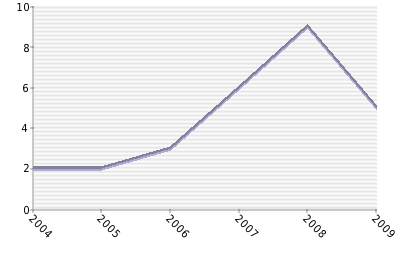
\includegraphics[scale=0.85]{img/soft-employees.png}
\end{figure}

En dépit de sa petite équipe, Soft Profile a réussi rester rentable et offrir des
services de haut gamme à tous ses clients.

\begin{figure}[h!]
	\centering
	\caption{\textcolor{blue}{Profit} - \textcolor{green}{Revenu} - \textcolor{red}{Dépenses} - \textcolor{yellow}{Dettes}}
	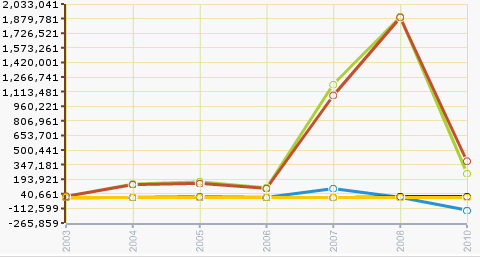
\includegraphics[scale=0.85]{img/soft-profit.png}
\end{figure}

En raison du fait que l'entreprise est principalement formé de jeunes gens, elle est très impliqué
dans les développements technologiques locales, souvent en offrant son siège pour accueillir des conférences,
marathons du hacking ou d'autres événements.

Dans le cadre de cet effort, elle est aussi une branche locale de CoworkingEU, un mouvement européen
qui favorise le partage de l'espace entre les personnes qui effectuent des activités individuelles
(ils ne travaillent pas sur le même projet et, souvent, ne savent même pas eux). La société
offre un environnement lucrative pour le travail de ces différentes personnes.

\section{Mon travail}

L'entreprise m'a donné l'opportunité de choisir le type de projet que je voulais faire,
étant donné qu'ils étaient spécialisés dans de nombreux domaines différents. Mon choix
était entre le travail sur une application web et la programmation de l'un des dispositifs
Vectron POS.

J'ai immédiatement choisi la programmation web, car ça était quelque chose que je
n'avais pas fait avant et il semblait plus intéressant que la programmation low-level
requis pour le dispositif POS. Pour ce projet, j'ai dû apprendre deux nouveaux langages
 de programmation et des nombreuses nouvelles technologies.

Le projet consistait en créer une petite application web qui offre l'accès en ligne aux
produits des nombreuses entreprises. L'application a \'et\'e destinée à l'administration de une
base de données, donc elle offre des moyens d'ajouter, modifier et supprimer des produits ou des
entreprises.

\begin{figure}[h!]
	\centering
	\caption{Structure de la base de données}
    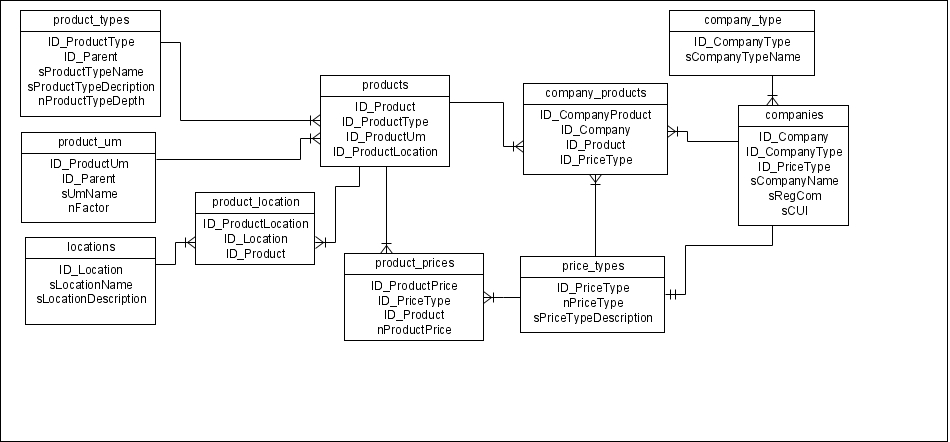
\includegraphics[scale=0.5]{img/project-database.jpg}
\end{figure}

Le défi s'est avéré être très intéressant que j'ai passé la première semaine d'apprentissage
sur les langages de programmation Python et JavaScript qui ont été nécessaires pour
rendre le frontend et le backend pour mon projet.

Le langage de programmation \textbf{Python} est largement utilisé dans le développement
web car il fournit des moyens faciles de prototypage de la fonctionnalité de l'application
et des constructions de haut niveau par rapport aux autres langages tels que C ou Java.
Python a été quelque chose que je n'avais pas appris à l'école et il a offert de façon
très différente de programmation que ce que j'étais habitué. En dépit de tout cela,
il s'est avéré être une langage très bon pour construire mon projet.

L'autre langage j'ai dû apprendre a été \textbf{JavaScript}. JavaScript est probablement le langage
le plus utilisée sur l'Internet. Contrairement à Python, il est utilisé dans les sites
et non sur les serveurs, donnant accès à des bases de données et autres services du système.
JavaScript a été plus facile d'apprendre car il ressemblait à C (lequel j'avais déjà fait \`a l’école)
tout en ajoutant des concepts de langages tels que Python avec lequel j'étais déjà familier.

La deuxième semaine a ensuite été consacré à l'apprentissage des cadres nécessaires
pour construire l'application: Django, un framework web écrit en Python, et ExtJS,
un framework écrit en JavaScript, utilisé pour construire le site réel.

\begin{figure}[ht!]
    \centering
	\caption{Prototype de l'interface utilisateur}
	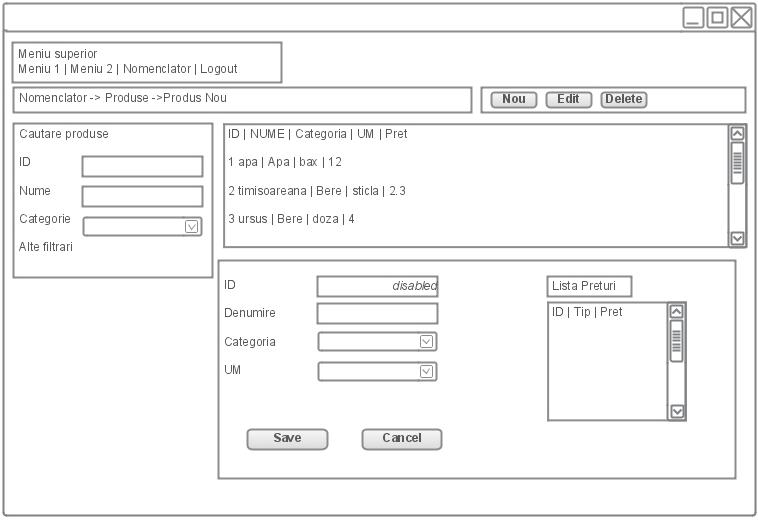
\includegraphics[scale=0.5]{img/ui.jpg}
\end{figure}

Les deux cadres utilisés pour la construction de l'application ont été très différents
dans leur but, tout comme les langages dans lesquelles ils ont été écrites.

Le \textbf{Framework Web Django} offert l'accès facile à une base de données, le déploiement
d'un serveur web et d'autres fonctionnalités essentielles à un site Web. Django
est un très complet de fonctionnalités par rapport à la plupart des autres cadres,
tout en conservant la vitesse et la facilité d'utilisation.

Le \textbf{Framework ExtJS} a été utilisé pour créer le site Web utilisé pour accéder
à des données fournies par Django. Contrairement à la plupart des sites Web, un site
web construit avec ExtJS ressemble à une application de bureau plus qu'un site web.
Cela a été très utile dans notre application, car nous avons eu un accès facile aux
choses telles que des boutons, tableaux, dialogues et ainsi de suite. Il a également
donné un sens plus professionnel sur le site, ce qui était approprié considérant son
rôle administratif.

Même si mon projet était complet après les deux premières semaines, j'ai décidé de
rester une semaine de plus et d'améliorer mon code et d'offrir la documentation pour
toutes mon travail. C'était aussi une étape très importante car, même si l'application
était fonctionnel, mon code a eu beaucoup de place à amélioration. Les autres employés
se sont avéré être très gentils pour m'aider à comprendre mes erreurs et offrir des conseils
sur la façon dont cela devrait être fait.

\chapter*{Conclusion}
\addcontentsline{toc}{chapter}{Conclusion}

Même si mon projet n'a pas eu un caractère officiel, car il était juste un exercice d'entraînement,
il a été une très bonne expérience d'apprentissage dans le monde de l'entreprise.

Toutes les nouvelles technologies que j'ai appris pendant mon stage à Soft Profile sont
révélés très utiles dans mon troisième année du licence car ils m'ont donné un avantage
sur la plupart de mes collègues qui n'avaient pas eu la chance d'étudier de nouveaux langages et paradigmes.

Une des choses les plus importantes que j'ai appris c'est que l'environnement dans
une entreprise n'a pas besoin être austère, il peut être très amicale et inspirante.
J'espère que l'entreprise pour laquelle je travaillerai va avoir certains de la même
mentalité que celle-ci.
\end{document}
